\documentclass[sigconf]{acmart}
% defining the \BibTeX command - from Oren Patashnik's original BibTeX documentation.
\def\BibTeX{{\rm B\kern-.05em{\sc i\kern-.025em b}\kern-.08emT\kern-.1667em\lower.7ex\hbox{E}\kern-.125emX}}
% Remove the annoying stuff
\settopmatter{printacmref=false} % Removes citation information below abstract
\renewcommand\footnotetextcopyrightpermission[1]{} % removes footnote with conference information in first column
\pagestyle{plain} % removes running headers



\usepackage{Nikolai}





\begin{document}

%
% The "title" command has an optional parameter, allowing the author to define a "short title" to be used in page headers.
\title{CMIS Hand-in 4: Finite Element Method}

\author{Nikolai Plambech Nielsen}
\email{lpk331@alumni.ku.dk}
\affiliation{%
  \institution{Niels Bohr Institute, University of Copenhagen}
}


\maketitle

\section{Finite Element Method}
The essence of the finite element method is to represent the domain as a finite set of elements (hence the name), and compute an approximate solution for each of these elements, adding up to the global solution. The actual elements vary on the dimensionality of the system. Straight-line segments for 1D problems, triangles for 2D and tetrahedra for 3D are the ones we focus on here due to their simplicity, but others can be used as well.

The actual method can be summarised in a series of steps:
\begin{enumerate}
	\item Convert the differential equation to a volume integral
	\item Define the elements
	\item Choose a shape and trial function for the elements
	\item Compute the elementwise integrals
	\item Assemble the global matrix and source vector
	\item Apply boundary conditions
	\item Compute the solution
\end{enumerate}
In this hand-in we focus on implementing the method in 1D and 2D, and use it to solve the Poisson equation for a simple source term:
\begin{equation}\label{key}
	\grad^2 u = c
\end{equation}
where to begin with we set $ c=0 $, and later $ c\in \mathbb{R} $. 

In the first step of the recipe we multiply each side by a function $ v(\V{r}) $, which must be continuously differentiable and 0 on the boundary of the domain ($ v(\V{r})=0,\ \forall \ \V{r}\in \Gamma $). Then we integrate over the domain on both sides to get
\begin{equation}\label{key}
	\int_{\Omega} v(\V{r}) \grad^2 u(\V{r}) \ud \Omega = \int_{\Omega} v(\V{r}) c \ud x
\end{equation}
This formulation of the problem is still equivalent to the original form, and is called ``Strong Form''. Next we perform integration by parts on the left hand side:
\begin{equation}\label{key}
	\int_{\Omega} v(\V{r}) \grad^2 u(\V{r}) \ud \Omega = \int_{\Gamma} v(\V{r}) \grad u(\V{r}) \ud \Gamma - \int_{\Omega} \grad v(\V{r}) \grad u(\V{r}) \ud \Omega
\end{equation}
But the first term is zero by definition, leading to the ``Weak Form'' of the problem:
\begin{equation}\label{key}
\int_{\Omega} \grad v(\V{r}) \grad u(\V{r}) \ud \Omega =- \int_{\Omega} v(\V{r}) c \ud x
\end{equation}
This takes care of the first step. In the second step we use the methods from last weeks hand-in on the generation of computational meshes. In particular I define the geometry of the setup in a \texttt{.poly} file and relegate the mesh generation to the \texttt{Triangle} program written by J. R. Shewchuk.

For the third step we approximate the unknown $ u $ by the function
\begin{equation}\label{key}
	u \approx \sum_{e\in \Omega} \V{N}^e \hat{u}^e,
\end{equation}
where the sum runs over all elements in the system, $ \hat{u}^e $ is a vector of the value of $ u $ on the 3 vertices in the $ e $'th element (with vertices counted counter clockwise): $ \hat{u}^e  = [u_i^e \ u^e_j \ u^e_k]^T $, and $ \V{N}^e $ is the ``shape function'' for the element. The shape function must have the following properties
\begin{equation}\label{key}
	N_i(\V{r}) = \begin{cases}
	1 & \V{r} = \V{r}_i, \\ 0, & \V{r}_j \land j \neq i
	\end{cases}, \quad \sum_{i} N_i(\V{r}) = 1.
\end{equation}
The first ensures proper interpolation for the points, whilst the second ensures that the approximation of $ \V{u} $ is exact on all vertices in the system. In one dimension we use a hat-function:
\begin{equation}\label{key}
	N_i(x) = \max\pp{0, 1- \vv{\frac{x_i - x}{\Delta x}}}
\end{equation}
which are 1 on the $ i $'th vertex, and 0 on all other (assuming equal spacing of nodes in the domain $ \Delta x $). And for triangles in two dimensions we use barycentric coordinates:
\begin{equation}\label{key}
	N_i^e(\V{r}) = \frac{A_i^e}{A^e}
\end{equation}
where the geometry is as seen in figure \ref{fig:barycentric}.
\begin{figure}
	\centering
	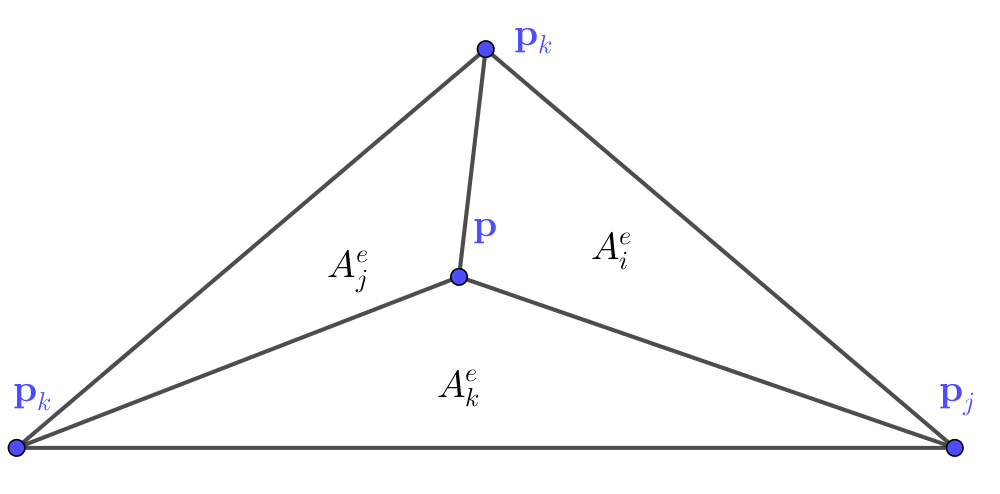
\includegraphics[width=0.7\linewidth]{barycentric.png}
	\caption{Barycentric coordinates for a triangular element.}
	\label{fig:barycentric}
\end{figure}
Where the areas can be found as the magnitudes of cross products:
\begin{equation}\label{key}
	N_i^e = \frac{\vv{(\V{p}_k - \V{p}_j) \times (\V{p}-\V{p}_j)}}{2 A^e}, \quad A^e = \frac{1}{2} \vv{(\V{p}_j - \V{p}_i) \times (\V{p}_k - \V{p}_i)}
\end{equation}
Now, the points of the triangles are two dimensional, so the cross products are also just the determinant of the $ 2 \times 2 $ matrix $ [(\V{p}_k - \V{p}_j),  \ (\V{p}-\V{p}_j) $ and equivalently for the total area, and other barycentric coordinates.



\end{document}
